\dots
\newpage

\usetikzlibrary{positioning, calc}

\chapter{Lecture 24/03/2025}

\section{Max Plus}

In what follows our task will be, given a joint density 𝑝(𝑥), to find the
tuple 𝑥𝑀 = argmax𝑥 𝑝(𝑥) (i.e. find a setting of the variables that has the
largest probability and the value of that probability).

To do so, we will use the max-plus algorithm.

As an example, consider a chain structure described by a Markov Random Field:

\tikzset{latent/.style={draw, circle}}
\begin{figure}[H]
\centering
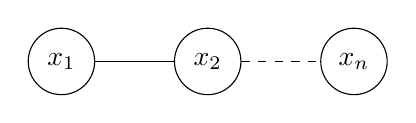
\begin{tikzpicture}
  \node[latent] (x1) {$x_1$};
  \node[latent, right=of x1] (x2) {$x_2$};
  \node[latent, right=of x2] (xn) {$x_n$};
  \draw (x1) -- (x2);
  \draw[dashed] (x2) -- (xn);
\end{tikzpicture}
\end{figure}

whose factorization reads as

$$
p(x) = \dfrac 1Z \psi_{1,2}(x_1, x_2) \dots \psi_{n-1,n}(x_{n-1}, x_n)
$$

Our goal is to mazimise p(x) w.r.t. $x_n$.

It is possible to distribute the factorization so that only local computations are required:

$$
\max_x p(x) = \max_{x_1} \dots \max_{x_2} p(x) = \dfrac 1Z \max_{x_1} \max_{x_2} \psi_{1,2}(x_1, x_2) \cdots \max_{x_{n-1}} \Psi _{n-2, n-1}(x_{n-2}, x_{n-1}) \max_{x_n} \psi_{n-1,n}(x_{n-1}, x_n)
$$

This happens because of the distributive properties of the max, indeed it
holds that, given $a > 0$:

\begin{itemize}
	\item the max distributes over the product:
	
	$$
	\max(ab, ac) = a \max(b, c)
	$$

	\item the max distributes over the sum:

	$$
	\max(a + b, a + c) = a + \max(b, c)
	$$

\end{itemize}

This allows us to take an approach similar to the one used in the sum-product algorithm.

Actually we will maximize $\log p(x)$, hence turning the product into sum of logarithms (and this justifies the name max-plus), i.e. our objective is to maximize

$$
\log p(x) = \sum_i \log \psi_i(x_i, x_{i+1}) - \log Z
$$

This saves us from product of factors that are possibly very small, since they are probabilities.

Max-plus algorithm is very similar to sum-product: essentially max replaces sum and plus replaces product. This leads to the following scenarios:

\tikzset{
  latent/.style={
    circle, draw=black,
    minimum size=24pt,
    align=center
  },
  function/.style={
    rectangle, draw=black, fill=gray!20,
    minimum width=16pt, minimum height=16pt,
    align=center
  }
}

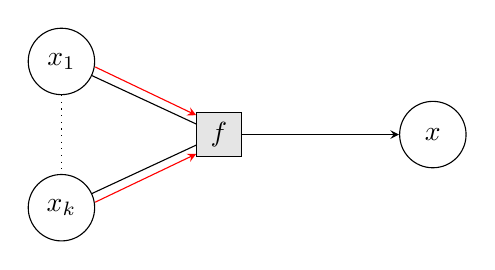
\begin{tikzpicture}[>=stealth]

  % x_1 at (0,0)
  \node[latent] (x1) {$x_1$};
  
  % x_k 2cm below x_1
  \node[latent, below= of x1] (xk) {$x_k$};
  
  % Dotted line between x_1 and x_k
  \draw[dotted] (x1) -- (xk);

  % f placed halfway between x_1 and x_k vertically, but shifted 2cm to the right
  \node[function] (f) at ($(x1)!0.5!(xk) + (2,0)$) {$f$};

  % x placed further right of f
  \node[latent, right=2cm of f] (x) {$x$};

  %--- Black + Red lines from x_1 to f ---
  % Black base (no arrow)
  \draw (x1) -- (f);
  % Red arrow slightly above
  \draw[->, red]
    ([yshift=-2pt] x1.east)  -- ([yshift=7pt] f.west);

  %--- Black + Red lines from x_k to f ---
  % Black base (no arrow)
  \draw (xk) -- (f);
  % Red arrow slightly below
  \draw[->, red]
    ([yshift=2pt] xk.east) -- ([yshift=-7pt] f.west);

  %--- Output arrow from f to x (black) ---
  \draw[->] (f) -- (x);

\end{tikzpicture}

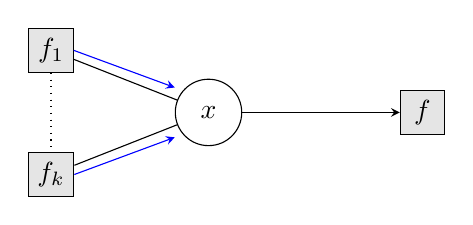
\begin{tikzpicture}[>=stealth]

	% x_1 at (0,0)
	\node[function] (f1) {$f_1$};
	
	% x_k 2cm below x_1
	\node[function, below= of f1] (fk) {$f_k$};
	
	% Dotted line between x_1 and x_k
	\draw[dotted] (f1) -- (fk);
  
	% f placed halfway between x_1 and x_k vertically, but shifted 2cm to the right
	\node[latent] (x) at ($(f1)!0.5!(fk) + (2,0)$) {$x$};
  
	% x placed further right of f
	\node[function, right=2cm of x] (f) {$f$};
  
	%--- Black + Red lines from x_1 to f ---
	% Black base (no arrow)
	\draw (f1) -- (x);
	% Red arrow slightly above
	\draw[->, blue]
	  ([yshift=-0pt] f1.east)  -- ([yshift=9pt] x.west);
  
	%--- Black + Red lines from x_k to f ---
	% Black base (no arrow)
	\draw (fk) -- (x);
	% Red arrow slightly below
	\draw[->, blue]
	  ([yshift=0pt] fk.east) -- ([yshift=-9pt] x.west);
  
	%--- Output arrow from f to x (black) ---
	\draw[->] (x) -- (f);
  
  \end{tikzpicture}

\section{Inference in general Probabilistic Graphical Models}

In what follows, we want to extend what we have seen so far to general probabilistic graphical models, meaning Factor Graphs which contain loops.

In these cases, we cannot identify the root and the leaves, hence we don't have well defined forward and backward directions.

\vspace{0.5em}

There are several possibilities:

\begin{itemize}
	\item \textbf{Junction Tree Algorithm}: it roughly builds a tree over the cliques of the Factor Graph, then exact inference is done in this tree. The worst case complexity of this algorithm is exponential in the sizeof the largest clique (so possibly very heavy computationally);
	\item \textbf{Loopy Belief Propagation}: forward and backward pass of the 	sum-product algorithm are iterated several times, until a fix point is reached. Unfortunately there is no guarantee that the algorithm	will converge. When it does, it provides an approximate answer to	the inference problem;
	\item \textbf{Monte Carlo Sampling}: a general strategy for approximate inference based on Sampling
	\item \textbf{Variational Inference}: it approximates the posterior distribution with a simpler distribution belonging to a pre-specified (parametric) class, which is the closer one to the true posterior, minimizing the KL-divergence.
\end{itemize}

\chapter{Hidden Markov Models}

In what follows our goal is to model \bfit{sequential data} (i.e. \bfit{time series}). This kind of data are observed from a process evolving in time, typically
at different time steps $x_1 , x_2 , . . . , x_N$ (i.e. assuming a discrete model of time). Since sequential data often arise through measurement of time series, there is correlation between observations at different time steps.

These data can come from very different domains: financial data, weather
forecast data, speech data, epidemiological data.

Markov Chains are natural models for sequential data, the following is a Markov chain of order 1:

\begin{center}
	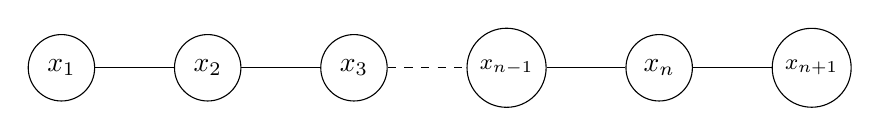
\begin{tikzpicture}
		\node[latent] (x1) {$x_1$};
	\node[latent, right=of x1] (x2) {$x_2$};
	\node[latent, right=of x2] (x3) {$x_3$};
	\node[latent, right=of x3] (xnm1) {\footnotesize $x_{n\text{\tiny-1}}$};
	\node[latent, right=of xnm1] (xn) {$x_{n}$};
	\node[latent, right=of xn] (xnp1) {\footnotesize $x_{n\text{\tiny+1}}$};
	\draw (x1) -- (x2);
	\draw (x2) -- (x3);
	\draw[dashed] (x3) -- (xnm1);
	\draw (xnm1) -- (xn);
	\draw (xn) -- (xnp1);
	\end{tikzpicture}
\end{center}

Since all the points (up to a certain step $N$) are observed, the factorization implied by the model is:

$$
p(x_1, \dots, x_N) = p(x_1) p(x_2 | x_1) \dots p(x_N | x_{N-1})
$$

It holds that future observations are independent of all but the most recent observation:

\newcommand{\Perp}{\perp\!\!\!\!\perp}

$$
x_{n+1} \Perp x_{n-1} | x_n
$$

A time homogeneous process is a process whose transition probability does not change in time, i.e. such that $p(x_n|x_{n-1}) = p(x_2|x_1)$.

These chains are not always the best model for describing sequential observations, indeed often there is a deeper dependency on the past, and first-order Markov chains suffer from too short memory.

In these cases, we can move to Markov models of order $k$, where the dependency of $x_n$ is on the previous $k$ steps. The following is a second-order Markov chain:

\begin{center}
	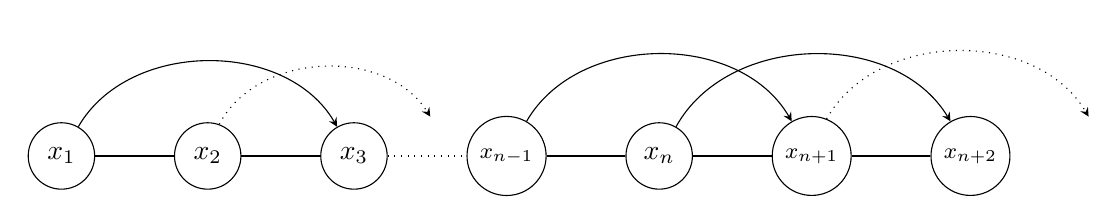
\begin{tikzpicture}[node distance=1cm and 1cm, >=stealth]
		\node[latent] (x1) {$x_1$};
		\node[latent, right=of x1] (x2) {$x_2$};
		\node[latent, right=of x2] (x3) {$x_3$};
		\node[latent, right=of x3] (xnm1) {\footnotesize $x_{n\text{\tiny-1}}$};
		\node[latent, right=of xnm1] (xn) {$x_{n}$};
		\node[latent, right=of xn] (xnp1) {\footnotesize $x_{n\text{\tiny+1}}$};
		\node[latent, right=of xnp1] (xnp2) {\footnotesize $x_{n\text{\tiny+2}}$};
		
		\draw (x1) -- (x2);
		\draw (x2) -- (x3);
		\draw[dotted] (x3) -- (xnm1);
		\draw (xnm1) -- (xn);
		\draw (xn) -- (xnp1);
		\draw (xnp1) -- (xnp2);
		
		\draw[->] (x1) to[bend left=60] (x3);
		\draw[->, dotted] (x2) to[bend left=60] ($($(x3)!0.5!(xnm1)$)+(0,0.5)$);
		\draw[->] (xnm1) to[bend left=60] (xnp1);
		\draw[->] (xn) to[bend left=60] (xnp2);
		\draw[->, dotted] (xnp1) to[bend left=60] ($(xnp2)!0.5!($(xnp2)+(3cm,1)$)$);
	\end{tikzpicture}
\end{center}

In this case the factorization of the joint probability distribution is:

$$
p(x_1, \dots, x_N) = p(x_1) p(x_2 | x_1) p(x_3 | x_1, x_2) \dots p(x_N | x_{N-2}, x_{N-1})
$$

And it holds that:

$$
x_{n+2} \Perp x_{n-1} | x_{n}, x_{n+1}
$$

\begin{observationblock}
	If $x_i$ are discrete, we talk about \bfit{Markov Chains}. If $x_i$ are continuous and $p(x_n|\dots)$ are Gaussian, we talk about \bfit{autorergressive models} (of order $k$).
\end{observationblock}

If we want to build a model for sequential data that is not limited by the Markov assumption of any order, we can rely on state space models, which introduce latent variables. In terms of graphical model, we have that latent variables form a Markov chain, and each of them corresponds to an observation:

\begin{center}
	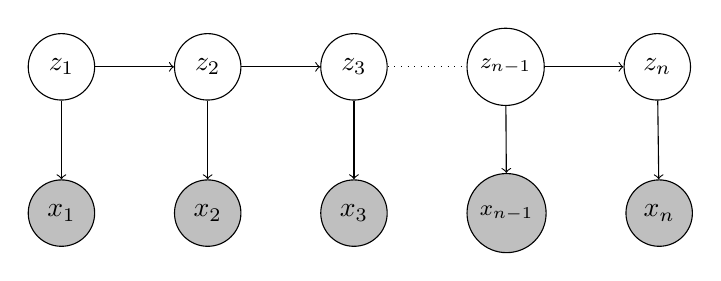
\begin{tikzpicture}
		\node[latent] (z1) {$z_1$};
		\node[latent, right=of z1] (z2) {$z_2$};
		\node[latent, right=of z2] (z3) {$z_3$};
		\node[latent, right=of z3] (znm1) {\footnotesize $z_{n\text{\tiny-1}}$};
		\node[latent, right=of znm1] (zn) {$z_{n}$};
		\draw[->] (z1) -- (z2);
		\draw[->] (z2) -- (z3);
		\draw[dotted] (z3) -- (znm1);
		\draw[->] (znm1) -- (zn);
		
		\node[latent, below=of z1, fill=lightgray] (x1) {$x_1$};
		\node[latent, right=of x1, fill=lightgray] (x2) {$x_2$};
		\node[latent, right=of x2, fill=lightgray] (x3) {$x_3$};
		\node[latent, right=of x3, fill=lightgray] (xnm1) {\footnotesize $x_{n\text{\tiny-1}}$};
		\node[latent, right=of xnm1, fill=lightgray] (xn) {$x_{n}$};
		\draw[->] (z1) -- (x1);
		\draw[->] (z2) -- (x2);
		\draw[->] (z3) -- (x3);
		\draw[->] (znm1) -- (xnm1);
		\draw[->] (zn) -- (xn);
	\end{tikzpicture}
\end{center}